%-----------------------------------------------------------------------------
%
%               Template for sigplanconf LaTeX Class
%
% Name:         sigplanconf-template.tex
%
% Purpose:      A template for sigplanconf.cls, which is a LaTeX 2e class
%               file for SIGPLAN conference proceedings.
%
% Author:       Paul C. Anagnostopoulos
%               Windfall Software
%               978 371-2316
%               paul@windfall.com
%
% Created:      15 February 2005
%
%-----------------------------------------------------------------------------

% \documentclass[tfpsymp,pagenumbers]{tfp07symp}

\documentclass{llncs}

% The following \documentclass options may be useful:
%
% 10pt          To set in 10-point type instead of 9-point.
% 11pt          To set in 11-point type instead of 9-point.
% authoryear    To obtain author/year citation style instead of numeric.

\usepackage{comment,amsmath,graphicx,color,url,hyperref}

\newcommand{\Ocaml}{OCaml}
\newcommand{\functory}{\textsf{Functory}}
%\newcommand{\JoCaml}{Jo{\&\!}Caml}
\newcommand{\unix}{\textsc{Unix}}

\begin{document}

\title{Functory: A Distributed Computing Library \\ for Objective Caml 
\thanks{This
    research was partly supported by the French national project U3CAT
    (\emph{Unification of Critical C Code Analysis Techniques},
    ANR-08-SEGI-021).}}

\author{Jean-Christophe Filli\^{a}tre and K. Kalyanasundaram}
\authorrunning{J.-C. Filli\^atre \and K. Kalyanasundaram}

\institute{CNRS, LRI, Univ Paris-Sud 11, Orsay F-91405\\
  INRIA Saclay - \^{I}le-de-France, ProVal, Orsay, F-91893 \\
   \email{filliatr@lri.fr, kalyan.krishnamani@inria.fr}}

\maketitle

\begin{abstract}
  We present Functory, a distributed computing library for
  Objective Caml. The main features of this library
  include (1) a polymorphic API, (2) several implementations to
  adapt to different deployment scenarios such as sequential,
  multi-core or network, and (3) a reliable fault-tolerance mechanism.
  This paper describes the motivation behind this work, as well as
  the design and implementation of the library. It also demonstrates
  the potential of the library using realistic experiments.
\end{abstract}

% PLAN
% 1. introduction, including related work
% 2. API
%    2.1 low level, compute, derived APIs
%    2.2 five different implementations
% 3. implementation
%    3.1 marshaling
%    3.2 protocol
%    3.3 fault tolerance
% 4. experiments

\section{Introduction}

% TODO
% Our library, \functory, is implemented in \Ocaml\ and is available
% from \url{http://www.lri.fr/~filliatr/functory/}.

This paper introduces \functory, a generic library for distributed
computing for a widely used functional programming language,
Objective Caml (\Ocaml\ for short). 
This work was initially motivated by the computing needs that
exist in our own research team. Our applications include large-scale
deductive program verification, which amounts to checking the validity
of a large number of logical formulas using a variety of automated
theorem provers~\cite{filliatre07cav}. Our computing infrastructure
consists of a few powerful multi-core machines (typically 8 to 16
cores) and several desktop PCs (typically dual-core). However, for our
application needs, no existing library provides a polymorphic API with
usual map/fold higher-order operations, built-in fault-tolerance, and
the ability to easily switch between multi-core and network
infrastructures.
Hence we designed and implemented such a library, which is
the subject of this paper.  
The library is available at 
\href{http://functory.lri.fr/}{\url{http://functory.lri.fr/}}.

The distributed computing library presented in this paper is not a
library that helps in parallelizing computations. Rather, it provides
facilities for reliable, distributed execution of parallelizable
computations. In particular, it provides a set of user-friendly APIs
that allows distributed execution of large-scale parallelizable
computations, very relevant to our application needs (and also
relevant to a variety of real-world applications). Further, the
distributed execution could be over multiple cores in the same machine
or over a network of machines. The most important features of our
library are the following:
\begin{itemize}
\item \emph{Genericity}: 
  it allows various patterns of polymorphic computations;
\item \emph{Simplicity}: switching between multiple cores on the same
  machine and a network of machines is as simple as changing a couple
  of lines of code;
\item \emph{Task distribution and fault-tolerance}: 
  it provides automatic task distribution and
  a robust fault-tolerance mechanism, thereby
  relieving the user from implementing such routines.
\end{itemize}
The application domain of such a distributed computing library is manyfold. 
It serves a variety of users and a wide spectrum of
needs, from desktop PCs to networks of machines.  Typical applications
would involve executing a large number of computationally expensive tasks
in a resource-optimal and time-efficient manner. This is also the case
in our research endeavours, that is validating thousands of
verification conditions using automated theorem provers, utilizing the
computing infrastructure to the maximum.
It is worth noting that 
\functory\ is not targeted at applications running on server farms,
crunching enormous amounts of data, such as Google's
MapReduce~\cite{mapreduce}.  

% what it is and what it is not
% \begin{itemize}
% \item it is not a library which does parallelization
% \item it is a library for reliable distributed execution of
%   parallelizable computation 
% \end{itemize}
% inspired by Google's MapReduce~\cite{mapreduce} (itself inspired by functional
% programming, ironically) ;  however, there are differences:
% \begin{itemize}
% \item polymorphic, higher-order API
% \item more generic (cores/network)
% \item does not focus on association lists
% \item we don't have data locality (future work)
% \end{itemize}
% what is the target audience/applications: 
% for instance, use if automatic provers on thousands of verification
% conditions, on computing infrastructures which can be
% \begin{itemize}
% \item a single machine with multiple cores, possibly remote
% \item several machines, small or large in number, over a network
% \end{itemize}

\medskip

In the following, we introduce our approach to distributed
computing in a functional programming setting and distinguish it from
related work.

\paragraph{Distributed Computing.}
A typical distributed computing library, as \functory, provides the
following (we borrow some terminology from Google's
MapReduce):
\begin{itemize}
\item A notion of \emph{tasks} which denote atomic computations
  to be performed in a distributed manner; 
\item A set of processes (possibly executing on remote machines)
  called \emph{workers} that perform
  the tasks, producing results;
\item A single process called a \emph{master} which is in charge
  of distributing the tasks among the workers and managing results
  produced by the workers.
\end{itemize}
In addition to the above, distributed computing environments also
implement mechanisms for fault-tolerance, efficient storage, and
distribution of tasks. This is required to handle network failures
that may occur, as well as to optimize the usage of machines in the
network. Another concern of importance is the transmission of messages
over the network. This requires efficient 
\emph{marshaling} of data, that is encoding and decoding of data 
for transmission over different computing environments.  It is desirable to
maintain architecture independence while transmitting marshalled data,
as machines in a distributed computing environment often run on
different hardware architectures and make use of different software
platforms. For example, machine word size or endianness may be different
across machines on the network.

\paragraph{A Functional Programming Approach.}
Our work was initially inspired by Google's
MapReduce\footnote{Ironically, Google's approach itself was inspired
  by functional programming primitives.}. However, our functional
programming environment allows us to be more generic. 
The main idea behind our approach is that
workers may implement any polymorphic function:
\begin{ocaml}
  worker: 'a -> 'b
\end{ocaml}
where \of{'a} denotes the type of tasks and \of{'b} the type of results.
Then the master is a
function to handle the results together with
a list of initial tasks:
\begin{ocaml}
  master: ('a -> 'b -> 'a list) -> 'a list -> unit
\end{ocaml}
The function passed to the master is applied whenever a result is
available. The first argument is the task (of type \of{'a}) and the
second one its result (of type \of{'b}). 
It may in turn generate new tasks, hence the return type
\of{'a list}.  
The master is executed as long as there are pending tasks.

Our library makes use of \Ocaml's marshaling capabilities as much as
possible. Whenever master and worker executables are exactly the same,
we can marshal polymorphic values and closures. However, it is not
always possible to have master and workers running the same
executable. In this case, we cannot marshal closures anymore but we
can still marshal polymorphic values as long as the same version of
\Ocaml\ is used to compile master and workers. When different versions
of \Ocaml\ are used, we can no longer marshal values but we can still
transmit strings between master and workers. Our library adapts to all
these situations, by providing several APIs.

% \medskip 

% In the following, we discuss some related work in this domain and
% elucidate how \functory\ differs from the other approaches.

\paragraph{Related Work.}
In order to compare and better distinguish
\of{Functory} from others work with related goals and motivations, we can
broadly classify the related work in this domain into:
\begin{enumerate}
\item \textit{Distributed Functional Languages (DFLs)} --- functional
  languages that provide built-in primitives for
  distribution. Examples include ML5, JoCaml, Glasgow Distributed
  Haskell, Erlang, etc.
\item \textit{Libraries for existing functional languages} --- that
  could be readily used in order to avoid implementing details like
  task distribution, fault-tolerance, socket programming, etc.
\end{enumerate}
\functory\ belongs to the second category.
For reasons of completeness, though, we first describe some existing DFLs
related to functional programming.

JoCaml is one of the DFLs which provides communication primitives
(like channels) for facilitating transmission of
computations. However, it does not provide ready-made language
features for fault-tolerance, which is indispensable in a distributed
setting. The user has to include code for fault-tolerance, as already
demonstrated in some JoCaml
library~\cite{mandel2008}. ML5~\cite{ML5}, a variant of ML, is a
programming language for distributed computing, specialized for web
programming. It provides primitives for transferring control between
the client and the server, as well as low-level primitives for
marshaling the data. As in the case before, ML5 is a programming
language that offers primitives for code mobility, and the code for
distribution of computation and fault-tolerance has to be included by
the user.  ML5 implements type-safe marshaling and
\functory\ does not, though an existing type-safe marshaling library
could be used with \functory. 
% Basically, the task will be transmitted
% along with the corresponding type and on unmarshaling, it could be
% matched for the correct type.
Glasgow Distributed Haskell (GdH)~\cite{GdH} is a pure distributed
functional language that is built on top of Glasgow Haskell and
provides features for distributed computing. It is an extension of
both Glasgow Parallel Haskell, that supports only one process and
multiple threads and Concurrent Haskell that supports multiple
processes. It also offers features for fault-tolerance - error
detection and error recovery primitives in the
language. 

CamlP3l~\cite{camlP3l} mixes the features of functional programming
with predefined patterns for parallel computation to offer a parallel
programming environment. Again, it is a programming language offering
primitives for distributing computation to parallel processes and also
to merge the results from parallel executions. Erlang~\cite{erlang} is
a programming language which has features for distribution and 
fault-tolerance. In particular, it has features for task distribution and is
more well-known for its rich error detection primitives and the
ability to support hot-swapping. The error detection primitives of
Erlang allow nodes to monitor processes in other nodes and also
facilitate automatic migration of tasks in failed nodes to recovered
or active nodes.

Any DFL above could have been used to implement our library. 
Our motivation, though, was neither to implement our system using any
existing DFL nor to come up with a new DFL.
The goal of \of{Functory} is rather to provide the
users of an \emph{existing} general-purpose functional programming
language, namely \Ocaml, high-level 
user-friendly APIs that hide the messy details of task distribution
and fault-tolerance.
We now turn to distributed computing libraries for general purpose
functional languages and weed out the distinguishing features of
\of{Functory}.

There are several implementations of Google's MapReduce in functional
programming languages. But \of{Functory} was just inspired by Google's
MapReduce and is not exactly a MapReduce implementation. The
simplest difference comes from the very fact that \of{Functory} does not
operate on key/value pairs. 
% TODO other difference = absence of data locality
PlasmaMR~\cite{plasma} is an \Ocaml\ implementation of Google's
MapReduce on a distributed file system PlasmaFS. It is able to use
PlasmaFS to its advantage --- the ability of the file system to handle
large files and query functions that implement data locality to
optimize network traffic. However, PlasmaMR does not support 
fault-tolerance which is indispensable in any distributed computing
application.
% The Disco project~\cite{disco} is an implementation of
% Google's MapReduce in Erlang~\cite{erlang}.
Another MapReduce
implementation in \Ocaml\ is Yohann
Padioleau's~\cite{poor-man-mapreduce}.  It is built on
top of OCamlMPI~\cite{ocamlMPI}, while our approach uses a homemade
protocol for message passing. Currently, we have less flexibility
w.r.t. deployment of the user program than OCamlMPI; on the other
hand, we provide a more generic API together with fault-tolerance. We
feel that an indispensible need for any distributed computing library
is fault-tolerance, and using a homemade protocol enables us to
tune our implementation to our needs of fault-tolerance.

The iTask system~\cite{iTask} is a library for the functional language
`Clean' targeted at distributed workflow management. The library
provides a set of combinators (some of which perform map/fold
operations) that facilitate applications running in different nodes
of a distributed system to communicate, exchange information and
coordinate their computations in a type-safe manner.

\begin{comment}
Closest to the approach in this paper is Yohann Padioleau's MapReduce
implementation in \Ocaml~\cite{poor-man-mapreduce}.  It is built on
top of OCamlMPI~\cite{ocamlMPI}, while our approach uses a homemade
protocol for message passing.  Currently, we have less flexibility
w.r.t. deployment of the user program than OCamlMPI; on the other
hand, we provide a 
more generic API together with fault-tolerance.  There are other
distributed computing libraries on top of which one could implement
the library discussed in this paper. JoCaml~\cite{jocaml} is one of
them. However, JoCaml does not provide fault-tolerance, which is
indispensable in a distributed setting. The user has to include code
for fault-tolerance, as already demonstrated in some JoCaml
experiments~\cite{mandel2008}. 

There are other implementations of distributed computing in the
context of functional programming. One is the Disco
project~\cite{disco}, which implements exactly Google's MapReduce in
Erlang~\cite{erlang}. Our library, on the contrary, is not an \Ocaml\
implementation of Google's MapReduce.
There are other ways to exploit multi-core architectures. One of these
is data parallelism, which is also relevant in the functional
programming setting~\cite{parallel-haskell}. Our work
does not target data parallelism at all.

\medskip
The paper is organized as follows. 
Section~\ref{sec:API} describes the API of our library.
Section~\ref{sec:implem} gives implementation details, focusing
on marshaling, network protocol and fault-tolerance.
Then Section~\ref{sec:experiments} illustrates the
potential of the presented library through experimental evaluation. 
Finally, Section~\ref{sec:future} outlines some future work.

\end{comment}

%%%%%%%%%%%%%%%%%%%%%%%%%%%%%%%%%%%%%%%%%%%%%%%%%%%%%%%%%%%%%%%%%%%%%%%%%%%%%%
\section{API}\label{sec:API}

This section describes our API. 
We start from a simple API which is reduced to a single higher-order
polymorphic function.
Then we explain how this function is actually implemented in terms of
low-level primitives, which are also provided in our API.
Conversely, we also explain how the same function can
be used to implement high-level distribution functions for map and
fold operations. Finally, we explain how our API is
implemented in five different ways, according to five different deployment
scenarios. 

\subsection{A Generic Distribution Function}

The generic distribution function in our API follows the idea
sketched in the introduction. It has the following signature:
\begin{ocaml}
  val compute: 
    worker:('a -> 'b) -> 
    master:('a * 'c -> 'b -> ('a * 'c) list) -> ('a * 'c) list -> unit
\end{ocaml}
Tasks are pairs, of type \of{'a * 'c}, where the first component is
passed to the worker and the second component is local to the master.
The \ocaml{worker} function should be pure\footnote{We mean
  \emph{observationally pure} here but we allow exceptions to be
  raised to signal failures.} 
and is executed in parallel
in all worker processes. The function \ocaml{master}, on the
contrary, can be impure and is only executed sequentially in the master process.
The \ocaml{master} function typically stores results 
in some internal data structure.
Additionally, it may produce new tasks, as a list of type 
\of{('a * 'c) list}, which are then appended to the current set of
pending tasks.

% TODO if we have space for it: small example to show the use of 'c
% 
%   let array_map f a =
%     let h = Hashtbl.create 17 in
%     let master (_, i) y = Hashtbl.add h i y in
%     let tasks = ref [] in
%     for i = 0 to Array.length a - 1 do tasks := (a.(i), i) :: !tasks done;
%     compute ~worker:f ~master !tasks;
%     Array.init n (fun i -> Hashtbl.find h i)

\begin{comment}
\section{Illustrative Example}\label{sec:example}

Let us assume we need to compute a sum such as
\begin{displaymath}
  s(n) = \sum_{i=0}^{n}f(i)
\end{displaymath}
where $f$ is a pure and computationally expensive function.
We start with the sequential implementation provided by the library:
\begin{ocaml}
  open Sequential
\end{ocaml}
The idea is to test our code on small values of $n$ before
parallelizing the computation for larger values.
Let us assume that $f$ is implemented as a top-level \of{worker} function:
\begin{ocaml}
  let worker i = ...
\end{ocaml}
and that $n$ is obtained from the command line:
\begin{ocaml}
  let n = int_of_string Sys.argv.(1)
\end{ocaml}
The list of tasks is simply the list of integers $0,1,\dots,n$,
computed as follows:
\begin{ocaml}
  let tasks = 
    let l = ref [] in 
    for i = 0 to n do l := (i, ()) :: !l done; 
    !l
\end{ocaml}
Each task is actually a pair, where the second component contains
some information which is kept local to the master process.
It is irrelevant here and thus the value \of{()} of type \of{unit} is used.
The current sum is kept into a global reference \of{s}:
\begin{ocaml}
  let s = ref 0
\end{ocaml}
The master function receives a task \of{(i,())} together with its
result \of{fi} and simply adds \of{fi} to \of{s}. There is no new task
generated, hence the returned empty list.
\begin{ocaml}
  let master (i,()) fi = s := !s + fi; []
\end{ocaml}
Finally, the whole computation takes place when we call the
\of{compute} function:
\begin{ocaml}
  let () = compute ~worker ~master tasks
\end{ocaml}

Now, let us assume we want to make use of a 4-core machine to compute
$s(n)$. It is as easy as just replacing the very first line with
\begin{ocaml}
  open Cores
  let () = set_number_of_cores 4
\end{ocaml}
while the rest of the code remains unchanged.

Later, we may want to use a network of machines instead, for example
two machines called \texttt{orcus} and \texttt{belzebuth} with 4 and 8
cores respectively. Similar to the above, we just replace the first
lines with
\begin{ocaml}
  open Network
  let () = declare_workers ~n:4 "orcus"
  let () = declare_workers ~n:8 "belzebuth"
  open Same
\end{ocaml}
Here, \of{Same} is a module which is to be used when master and worker
are running the same executable. It provides a \of{compute} function
which has the same signature as in modules \of{Sequential} and
\of{Cores}, so that the rest of the code remains unchanged. Master and
worker processes are distinguished at runtime using an environment
variable \texttt{WORKER} which is set/unset.

If we need to write two different programs for master and worker, for
reason of binary incompatibility or any other reason, the library API
is providing functions to do that. If master and worker are still
compiled with the same version of \Ocaml, we use the \of{Poly} module
which provides a polymorphic API. Let us start with the worker program.
It is as simple as
\begin{ocaml}
  open Poly
  let worker i = ...
  let () = Worker.compute worker ()
\end{ocaml}
The \of{Worker.compute} function enters a loop which waits for
tasks sent by the master and returns results computed using \of{worker}.
The master program is almost the same as before. First, we replace
module \of{Same} with module \of{Poly}:
\begin{ocaml}
  open Network
  let () = declare_workers ~n:4 "orcus"
  let () = declare_workers ~n:8 "belzebuth"
  open Poly
\end{ocaml}
Tasks and \of{master} function are unchanged:
\begin{ocaml}
  let tasks = ...
  let s = ref 0
  let master (i,()) fi = ...
\end{ocaml}
Finally, we start the computation with \of{Master.compute}, which does
not have a \of{worker} parameter anymore:
\begin{ocaml}
  let () = Master.compute ~master tasks
\end{ocaml}

When master and worker programs are compiled with different
versions of the \Ocaml\ compiler, our library still provides
a monomorphic API over strings. As a consequence, we need to convert
integers to and from strings in both master and worker.
The modified worker program is as follows:
\begin{ocaml}
  open Mono
  let worker i = ...
  let worker_string i = string_of_int (worker (int_of_string i))
  let () = Worker.compute worker_string ()
\end{ocaml}
The master program is modified in a similar way.
We simply replace \of{Poly} with \of{Mono} and encode/decode integers
as strings, as follows:
\begin{ocaml}
  let tasks = 
    let l = ref [] in 
    for i = 0 to n do l := (string_of_int i, ()) :: !l done; 
    !l
  let master (i,()) fi = s := !s + int_of_string fi; []
\end{ocaml}
\end{comment}

\subsection{Low-level Primitives}

% motivation is finer control over task/workers/execution
% example 1: remove *some* tasks when others are completed
% example 2: interactive program (GUI, control, etc.)

The function \of{compute} above can actually be implemented in terms
of low-level primitives, such as adding a task, adding a worker,
performing some communication between master and workers, etc.
These primitives are provided in our API, such that the user can
interact with the execution of the distributed computation.  For
instance, a monitoring-like application can use these primitives to
allow observation and modification of resources (tasks, workers)
during the course of a computation.
A type for distributed computations is introduced:
\begin{ocaml}
  type ('a, 'c) computation
\end{ocaml}
A computation is created with a function \of{create}, which accepts
the same \of{worker} and \of{master} as \of{compute}:
\begin{ocaml}
  val create: worker:('a -> 'b) -> 
    master:('a * 'c -> 'b -> ('a * 'c) list) -> ('a, 'c) computation
\end{ocaml}
Contrary to \of{compute}, it takes no list of tasks and returns
immediately. Tasks can be added later using the following function:
\begin{ocaml}
  val add_task: ('a, 'c) computation -> 'a * 'c -> unit
\end{ocaml}
A function is provided to perform \emph{one step} of a given
computation:
\begin{ocaml}
  val one_step: ('a, 'c) computation -> unit
\end{ocaml}
Calling this function results in one exchange of messages between
master and workers: task assignments to workers, results returned to
the master, etc. A few other functions are provided, such as
\of{status} to query the status of a computation, \of{clear} to remove
all tasks, etc.

Using these low-level primitives, it is straightforward to implement
the \of{compute} function. Basically, it is as simple as the following:
\begin{ocaml}
let compute ~worker ~master tasks =
  let c = create worker master in
  List.iter (add_task c) tasks;
  while status c = Running do one_step c done
\end{ocaml}

\subsection{High-level API}\label{sec:derived}

In most cases, the easiest way to parallelize an execution is to make
use of operations over lists, where processing of the
list elements are done in parallel. 
To facilitate such a processing,
our library provides most commonly used list operations, all 
implemented using our generic \of{compute} function.

The most obvious operation is the traditional map operation over
lists, that is \of{val map: f:('a -> 'b) -> 'a list -> 'b list}.
Each task consists of the application of function \of{f} to a list element.
More interesting is a combination of map and fold operations.
For instance, we provide different flavors of function
\begin{ocaml}
  val map_fold: f:('a -> 'b) -> fold:('c -> 'b -> 'c) -> 'c -> 'a list -> 'c
\end{ocaml}
which, given two functions, an accumulator $a$ and a list $l$, computes
\begin{equation}\label{eq:map-fold}
  \of{fold} ... (\of{fold} (\of{fold} ~ a ~ (\of{f} ~ x_1)) (\of{f} ~ x_2))
  ... (\of{f} ~ x_n)
\end{equation}
for some permutation $[x_1,x_2,...,x_n]$ of the list $l$.
We assume that the \of{f} operations are always performed in parallel.
Regarding \of{fold} operations, we distinguish two cases:
either \of{fold} operations are computationally less expensive
than \of{f} and we perform them locally;
or \of{fold} operations are computationally expensive and we
perform them in parallel.
Thus we provide two functions \of{map_local_fold} and \of{map_remote_fold}.

In the case of \of{map_remote_fold}, only one \of{fold} operation can
be performed at a time (possibly in parallel with \of{f}
operations), as obvious from~(\ref{eq:map-fold}). However, there are
cases where several \of{fold} operations can be performed in parallel,
as early as intermediate results of \of{fold} operations are available.
This is the case when \of{fold} is an associative operation (which
implies that types \of{'b} and \of{'c} are the same).
Whenever
\of{fold} is also commutative, we can perform even more \of{fold}
operations in parallel. Thus our API provides two functions
\of{map_fold_a} and \of{map_fold_ac} for these two particular cases,
with types
\begin{ocaml}
  val map_fold_ac, map_fold_a: 
    f:('a -> 'b) -> fold:('b -> 'b -> 'b) -> 'b -> 'a list -> 'b 
\end{ocaml}
It is rather straightforward to derive these five functions from the
generic \of{compute} function; we invite readers interested in details to
refer to the source code.

\subsection{Deployment Scenarios}

Actually, our library provides not just one implementation for the API above,
but instead five different implementations
depending on the deployment scenario. 
The first two scenarios are the following: 
\begin{enumerate}
\item \textbf{Purely sequential execution:}
  this is mostly intended to be a reference implementation
  for performance comparisons, as well as for debugging;

\item \textbf{Several cores on the same machine:} 
  this implementation is intended to distribute the computation over a
  single machine and it makes use of \unix\ processes;
\end{enumerate}
The next three scenarios are intended for distributing the
computation over a network of machines.
\begin{enumerate}
\setcounter{enumi}{2}
\item \textbf{Same executable run on master and worker machines:}
  this implementation makes use of the ability to marshal \Ocaml\
  closures and polymorphic values.
%   Depending on whether the program is run as a master or as a worker,
%   the relevant arguments of \ocaml{compute} are used.

\item \textbf{Master and workers are different programs, compiled with
    the same version of \Ocaml:} 
  we can no longer marshal closures but we can still
  marshal polymorphic values. API functions are split into two sets,
  used to implement master and workers respectively.

\item \textbf{Master and workers are different programs, not even
    compiled with the same version of \Ocaml:} we can no
  longer use marshaling, so API functions are restricted to work on
  strings instead of polymorphic values.
\end{enumerate}
Our library is organized into three modules: \of{Sequential} for the
pure sequential implementation, \of{Cores} for multiple cores on the
same machine and \of{Network} for a network of machines, respectively.
The \of{Network} module itself is organized into three sub-modules,
called \of{Same}, \of{Poly} and \of{Mono},
corresponding to contexts 3, 4 and 5 above. 

\subsection{Several Libraries in One}

From  the description above, it is clear that our library provides
several APIs of different granularities, as well as several
implementations for various deployment scenarios. 
Most combinations are meaningful, resulting in
thirteen possible different ways of using our library.
For instance, one may use the low-level API on a single multi-core
machine, or use the high-level API on a network of machines all
running the same executable, etc.
From the implementation point of view, there is almost no code
duplication. We are using \Ocaml\ functors to derive specific
implementations from generic ones.

%%%%%%%%%%%%%%%%%%%%%%%%%%%%%%%%%%%%%%%%%%%%%%%%%%%%%%%%%%%%%%%%%%%%%%%%%%%%%%
\section{Implementation Details}\label{sec:implem}

The implementation of the \of{Sequential}
module is straightforward and does not require any explanation.
The \of{Cores} module is implemented with \unix\ processes, using
the \of{fork} and \of{wait} system calls provided by the \of{Unix}
library of \Ocaml. We do not describe this implementation but
rather focus on the more interesting module \of{Network}.

\begin{comment}
  \subsection{Multiple Cores}

  The \of{Cores} module implements the distributed computing library
  for multiple cores on the same machine.
  % As illustrated in Section~\ref{sec:example},
  It provides a function \of{set_number_of_cores: int -> unit} to
  indicate the number of cores to be used. The number passed to this
  function may be different from the actual number of cores in the
  machine; it is rather the number of tasks to be performed
  simultaneously.
  % TODO comment more on the number of cores?  Thus a program using
  % the \of{Cores} module typically begins with
  % \begin{ocaml}
  %   open Cores let () = set_number_of_cores 8
  % \end{ocaml}

  The \of{Cores} module is implemented with \unix\ processes, using
  the \of{fork} and \of{wait} system calls provided by the \of{Unix}
  library of \Ocaml. The idea is pretty simple.  The \of{compute}
  function maintains a global table of pending tasks and keeps track
  of the number of idle cores.  Whenever there is a pending task and
  an idle core, a new sub-process is created using \of{Unix.fork};
  once completed, the sub-process marshals the result into a local
  file. The main process maintains a table mapping each sub-process ID
  to the input task and the local file name. It waits for any
  completed sub-process using \of{Unix.wait} and recovers the result
  from the local file. Then function \of{master} is applied, which may
  generate new tasks.  The main loop can be depicted in the following
  way:
  \begin{flushleft}
    \quad  \textbf{while} pending tasks $\lor$ pending sub-processes \\
    \quad  \quad \textbf{while} pending tasks $\land$ idle cores \\
    \quad  \quad \quad create new sub-process for some task \\
    \quad  \quad \textbf{wait} for any completed sub-process \\
    \quad  \quad \quad push new tasks generated by \of{master} \\
  \end{flushleft}
  We also have an alternative implementation using \unix\ pipes
  instead of local files.

  The scheduling of tasks to the different cores is left to the
  operating system, through \of{Unix.fork}. Thus it may be the case
  that two tasks are executed on the same core, even if the declared
  number of cores is less or equal than the actual number of cores on
  the machine.
  % TODO: comment on user-provided scheduling?
\end{comment}

\subsection{Marshaling}

  As mentioned in Section~\ref{sec:API}, the \of{Network} module
  actually provides three different implementations as sub-modules, according to
  three different execution scenarios, the details of which are
  presented below:

  \paragraph{\of{Same}.} This module is used when master and workers
  are running the same executable. The master and workers have to be
  differentiated in some manner. We use an environment variable
  \texttt{WORKER} for this purpose. When set, it indicates that the
  executable acts as a worker. At runtime, a worker immediately
  enters a loop waiting for tasks from the master, without even
  getting into the user code.  As explained in Section~\ref{sec:API},
  the master function has the following signature.
  \begin{ocaml}
  val compute: worker:('a -> 'b) -> 
    master:('a * 'c -> 'b -> ('a * 'c) list) -> ('a * 'c) list -> unit
  \end{ocaml}
  The master uses marshaling to send both a closure of type \of{'a -> 'b} and a task of type \of{'a} to the worker. The resulting
  strings are passed as argument \of{f} and \of{x} in message
  \of{Assign}. Similarly, the worker uses marshaling to send back the
  result of the computation of type \of{'b}, which is the argument
  \of{s} in message \of{Completed}. These messages are described in
  detail in Section~\ref{sec:protocol}.

  Though the ability to run the same executable helps a lot in
  deploying the program in different machines, it comes at a small
  price. Since the worker is not getting into the user code, closures
  which are transmitted from the master cannot refer to global
  variables in the user code. Indeed, the initialization code for
  these global variables is never reached on the worker side. For
  instance, some code for drawing Mandelbrot's set
  could be written as follows:
  \begin{ocaml}
    let max_iterations = 200 
    let worker si = ... draw sub-image si using max_iterations ...
  \end{ocaml}
  That is, the global function \of{worker} makes use of the global
  variable \of{max_iterations}. The worker gets the function to
  compute from the master, namely the closure corresponding to
  function \of{worker} in that case, but on the worker side the
  initialization of \of{max_iterations} is never executed.

  One obvious solution is not to use global variables in the worker
  code. This is not always possible, though.  To overcome this, the
  \of{Same} sub-module also provides a \of{Worker.compute} function to
  start the worker loop manually from the user code. This way, it can
  be started at any point, in particular after the initialization of
  the required global variables.  Master and worker are still running
  the same executable, but are distinguished using a user-defined way
  (command-line argument, environment variable, etc.).

  There are situations where it is not possible to run the
  same executable for master and workers.  For instance, architectures
  or operating systems could be different across the network.  For
  that reason, the \of{Network} module provides two other
  implementations.

  \paragraph{\of{Poly}.} When master and workers are compiled with the
  same version of \Ocaml, we can no longer marshal closures but we can
  still marshal polymorphic values. Indeed, an interesting property of
  marshaling in \Ocaml\ is to be fully architecture-independent, as
  long as a single version of \Ocaml\ is used. It is worth pointing
  out that absence of marshaled closures now enables the use of two
  different programs for master and workers. This is not mandatory,
  though, since master and workers could still be distinguished at
  runtime as in the previous case.

  On the worker side, the main loop is started manually using
  \of{Worker.compute}. The computation to be performed on each task is
  given as an argument to this function. It thus looks as follows:
  \begin{ocaml}
    Worker.compute: ('a -> 'b) -> unit -> unit
  \end{ocaml}
  On the master side, the \of{compute} function is simpler than in the
  previous case, as it has one argument less, and thus has the
  following signature.
  \begin{ocaml}
    Master.compute: 
      master:('a * 'c -> 'b -> ('a * 'c) list) -> ('a * 'c) list -> unit
  \end{ocaml}
  For realistic applications, where master and workers are completely
  different programs, possibly written by different teams, this is the
  module of choice in our library, since it can still pass polymorphic
  values over the network. The issues of marshaling are automatically
  taken care of by the \Ocaml\ runtime.

  The derived API presented in Section~\ref{sec:derived} is adapted to
  deal with the absence of closures. Exactly as the \of{compute}
  function, each API now takes two forms, one for the master and
  another for the workers. For example, \of{map_fold_ac} takes the
  following forms.
  \begin{ocaml}
  Worker.map_fold_ac: f:('a -> 'b) -> fold:('b -> 'b -> 'b) -> unit 
  Master.map_fold_ac: 'b -> 'a list -> 'b
  \end{ocaml}
  It is the responsibility of the user to ensure consistency
  between master and workers.

  \paragraph{\of{Mono}.} When master and workers are compiled using
  different versions of \Ocaml, we can no longer use marshaling.  As
  in the previous case, we split \of{compute} into two functions, one
  for master and one for workers. In addition, values transmitted over
  the network can only be strings. The signature thus takes the
  following form.
  \begin{ocaml}
  Worker.compute: (string -> string) -> unit 
  Master.compute: master:(string * 'c -> string -> (string * 'c) list) -> 
    (string * 'c) list -> unit
  \end{ocaml}
  Any other datatype for tasks should be encoded to/from strings. This
  conversion is left to the user.  Note that the second component of
  each task is still polymorphic (of type \of{'c} here), since it is
  local to the master.

  % There is actually a single, generic implementation, which is then
  % instantiated in three different ways, corresponding to the three
  % scenarios.  The generic implementation assumes that only strings
  % are being transmitted over the network, as evident from the
  % \of{Assign} and \of{Completed} messages in
  % Section~\ref{sec:protocol}. Depending on the implementation, these
  % strings could be marshaled closures, marshaled values or simply
  % user strings.

\subsection{Protocol}\label{sec:protocol}

The \of{Network} module implements the distributed computing library
for a network of machines. 
% As illustrated in Section~\ref{sec:example}, 
It provides a function
\of{declare_workers: n:int -> string -> unit} to fill a table of
worker machines. 
% The argument \of{n} indicates the number of cores to
% be used in each worker machine, analogous to the \of{Cores}
% module. Thus a program using the \of{Network} module typically begins
% with
% \begin{ocaml}
% open Network
% let () = declare_workers ~n:12 "hostname1"
% let () = declare_workers ~n:8  "192.168.24.2"
% ...
% \end{ocaml}

The \of{Network} module is based on a traditional TCP-based client/server
architecture, where each worker is a server and the master is the
client of each worker. The main execution loop is similar to the one
in the \of{Cores} module, where distant processes on remote machines
correspond to sub-processes and idle cores are the idle cores 
of remote workers. 
The master is purely sequential. In particular, when running the user
\of{master} function, it is not capable of performing any task-related
computation. This is not an issue, as we assume the \of{master}
function not to be time-consuming.
The worker, on the other hand, forks a new process to execute the task
and hence can communicate with the master during its computation.
We subsequently describe issues of message
transfer and fault-tolerance.

%\subsubsection{Protocol}

Messages sent from master to workers could be any of the following kinds:
\begin{description}
\item[\of{Assign(id:int, f:string, x:string)}] This message assigns a
  new task to the worker, the task being identified by the unique
  integer \of{id}. The task to be performed is given by strings \of{f}
  and \of{x}, which are interpreted depending on the context.

\item[\of{Kill(id:int)}] This message tells the worker to kill the task
  identified by \of{id}.

\item[\of{Stop}] This message informs the worker about completion of
  the computation, so that it may choose to exit.

\item[\of{Ping}] This message is used to check if the worker is still
  alive, expecting a \of{Pong} message from the worker in return.
\end{description}
Messages sent by workers could be any of the following kinds:
\begin{description}
\item[\of{Pong}] This message is an acknowledgment for a \of{Ping}
  message from the master.

\item[\of{Completed(id:int, s:string)}] This message indicates the
  completion of a task identified by \of{id}, with result \of{s}.

\item[\of{Aborted(id:int)}] This message informs the master that the
  task identified by \of{id} is aborted, either as a response to a
  \of{Kill} message or because of a worker malfunction.
\end{description}
Our implementation of the protocol works across different
architectures, so that master and workers could be run on completely
different platforms w.r.t. endianness, version of \Ocaml\ and
operating system.

\subsection{Fault-Tolerance}\label{sec:fault}

The main issue in any distributed computing environment is the ability
to handle faults, which is also a distinguishing feature of our
library.  
The fault-tolerance mechanism of \functory\ is limited to workers;
handling master failures is the responsibility of the user, for
instance by periodically logging the master's state.
Worker faults are mainly of two kinds: either a worker is stopped,
and possibly later restarted; or a worker is temporarily or
permanently unreachable on the network. To provide fault-tolerance,
our master implementation is keeping track of the status of each
worker.  This status is controlled by two timeout parameters $T_1$ and
$T_2$ and \of{Ping} and \of{Pong} messages sent by master and workers,
respectively. There are four possible statuses for a worker:
\begin{description}
\item[\of{not connected}:] there is no ongoing TCP connection between
  the master and the worker;
\item[\of{alive}:] the worker has sent some message
  within $T_1$ seconds;
\item[\of{pinged}:] the worker has not sent any message within $T_1$
  seconds and the master has sent the worker a
  \of{Ping} message within $T_2$ seconds;
\item[\of{unreachable}:] the worker has not yet responded to the \of{Ping}
  message (for more than $T_2$ seconds).
\end{description}
Whenever we receive a message from a worker, its status changes to
\of{alive} and its timeout value is reset.
\begin{center}
  \includegraphics[scale=0.7]{state.mps}
\end{center}

Fault tolerance is achieved by exploiting the status of workers as
follows. First, tasks are only assigned to workers with either
\of{alive} or \of{pinged} status. Second, whenever a worker executing
a task $t$ moves to status \of{not connected} or \of{unreachable}, the
task $t$ is rescheduled, which means it is put back in the set of
pending tasks. Whenever a task is completed, any rescheduled copy of
this task is either removed from the set of pending tasks or killed if
it was already assigned to another worker.

It is worth noticing that our library is also robust w.r.t. exceptions
raised by the user-provided \of{worker} function. In that case, an
\of{Aborted} message is sent to the master and the task is
rescheduled. It is the responsibility of the user to handle such
exceptions if necessary.

% The signature for the generic
% implementation is therefore as follows:
% \begin{ocaml}
%   generic_master:
%     assign_job:('a -> string * string) ->
%     master:('a * 'c -> string -> ('a * 'c) list)  ->
%     ('a * 'c) list -> unit
% \end{ocaml}
% The first argument \of{assign_job} is a function indicating the two
% strings that are passed in the \of{Assign} message of the protocol.
% We can now distinguish the three cases, based on \of{assign_job}:
% \begin{description}
% \item[\of{Same}:] in this case, \of{assign_job} simply returns
%   the marshaled closure together with the marshaled value.
% \item[\of{Poly}:] in this case, \of{assign_job} is simply
%   returning the marshaled value (the first string being meaningless in
%   this context).
% \item[\of{Mono}:] in this case, \of{assign_job} is immediately
%   returning its argument (the first string being meaningless in
%   this context).
% \end{description}

%%%%%%%%%%%%%%%%%%%%%%%%%%%%%%%%%%%%%%%%%%%%%%%%%%%%%%%%%%%%%%%%%%%%%%%%%%%%%%
\section{Experiments}\label{sec:experiments}

In this section, we demonstrate the potential of using \functory\ on
several case studies.
The source code for all these case studies is contained in the
distribution, in sub-directory \texttt{tests/}.

The purpose of the following experiments is to compare the various
deployments, namely sequential, cores and network.
For this comparison to be fair, all
computations are performed on the same machine, an 8 core Intel Xeon
3.2 GHz running Debian Linux. The sequential implementation uses a
single core. The multi-core implementation uses up to 8 cores of
the machine. The network implementation uses 8 workers running locally and
a master running on a remote machine over a LAN 
(which incurs communication cost).

\subsection{N-queens}\label{sec:n-queens}

The first example is the classical $N$-queens problem, where we
compute the total number of ways to place $N$ queens on a $N\times N$
chessboard in such a way no two queens attack each other.
We use a standard backtracking algorithm for this problem, which
places the queens one by one starting from the first row.
Distributing the computation is thus quite easy: we consider all
possible ways to place queens on the first $D$ rows and then perform
the subsequent search in parallel. Choosing $D=1$ will result in
exactly $N$ tasks; choosing $D=2$ will result in $N^2-3N+2$ tasks; 
greater values for $D$ would result in too many tasks.

% TODO: make a picture to illustrate positioning of 2 queens on the
% first 2 rows

Each task only consists of three integers and its result is one integer,
which is the total number of solutions for this task.
We make use of function \of{map_local_fold} from the derived API,
where \of{f} is performing the search and \of{fold} simply adds the
intermediate results.
In the network configuration, we make use of the \of{Network.Same}
module, workers and master being the same executable.

The following table shows execution times for various values of $N$
and our three different implementations: \of{Sequential}, \of{Cores}, and
\of{Network}. The purpose of this experiment is to measure the speedup
w.r.t. the sequential implementation.
The first column shows the value of $N$.  The number of tasks is shown in
second column.  Then the last three columns show execution times in
seconds for the three implementations. The figures within brackets
show the speedup w.r.t. sequential implementation. Speedup ratios are
also displayed in Fig.~\ref{fig:queens} (note the logarithmic scale).
  \begin{center}
    \begin{tabular}{|r|r|r|r|r|r|}
      \hline
      N & D & \#tasks  & \of{Sequential}& \of{Cores}              & \of{Network} 
      \\\hline\hline
      16 &1&   16    &  15.2     &   2.04 (7.45$\times$) &  2.35  (6.47$\times$) 
      \\\hline
      &2&  210    &  15.2     &   2.01 (7.56$\times$) & 21.80  (0.69$\times$)
      \\\hline
      17 &1&   17    & 107.0     &  17.20 (6.22$\times$) & 16.20  (6.60$\times$)
      \\\hline
      &2&  240    & 107.0     &  14.00 (7.64$\times$) & 24.90  (4.30$\times$)
      \\\hline
      18 &1&   18    & 787.0     & 123.00 (6.40$\times$) & 125.00 (6.30$\times$)  
      \\\hline
      &2&  272    & 787.0     & 103.00 (7.64$\times$) & 124.00 (6.34$\times$)  
      \\\hline
      19 &1&   19    &6120.0     & 937.00 (6.53$\times$) & 940.00 (6.51$\times$)  
      \\\hline
      &2&  306    &6130.0     & 796.00 (7.70$\times$) & 819.00 (7.48$\times$)
      \\\hline
    \end{tabular}
  \end{center}
\begin{figure}[t]
  \vspace*{-4em}
  \begin{center}
    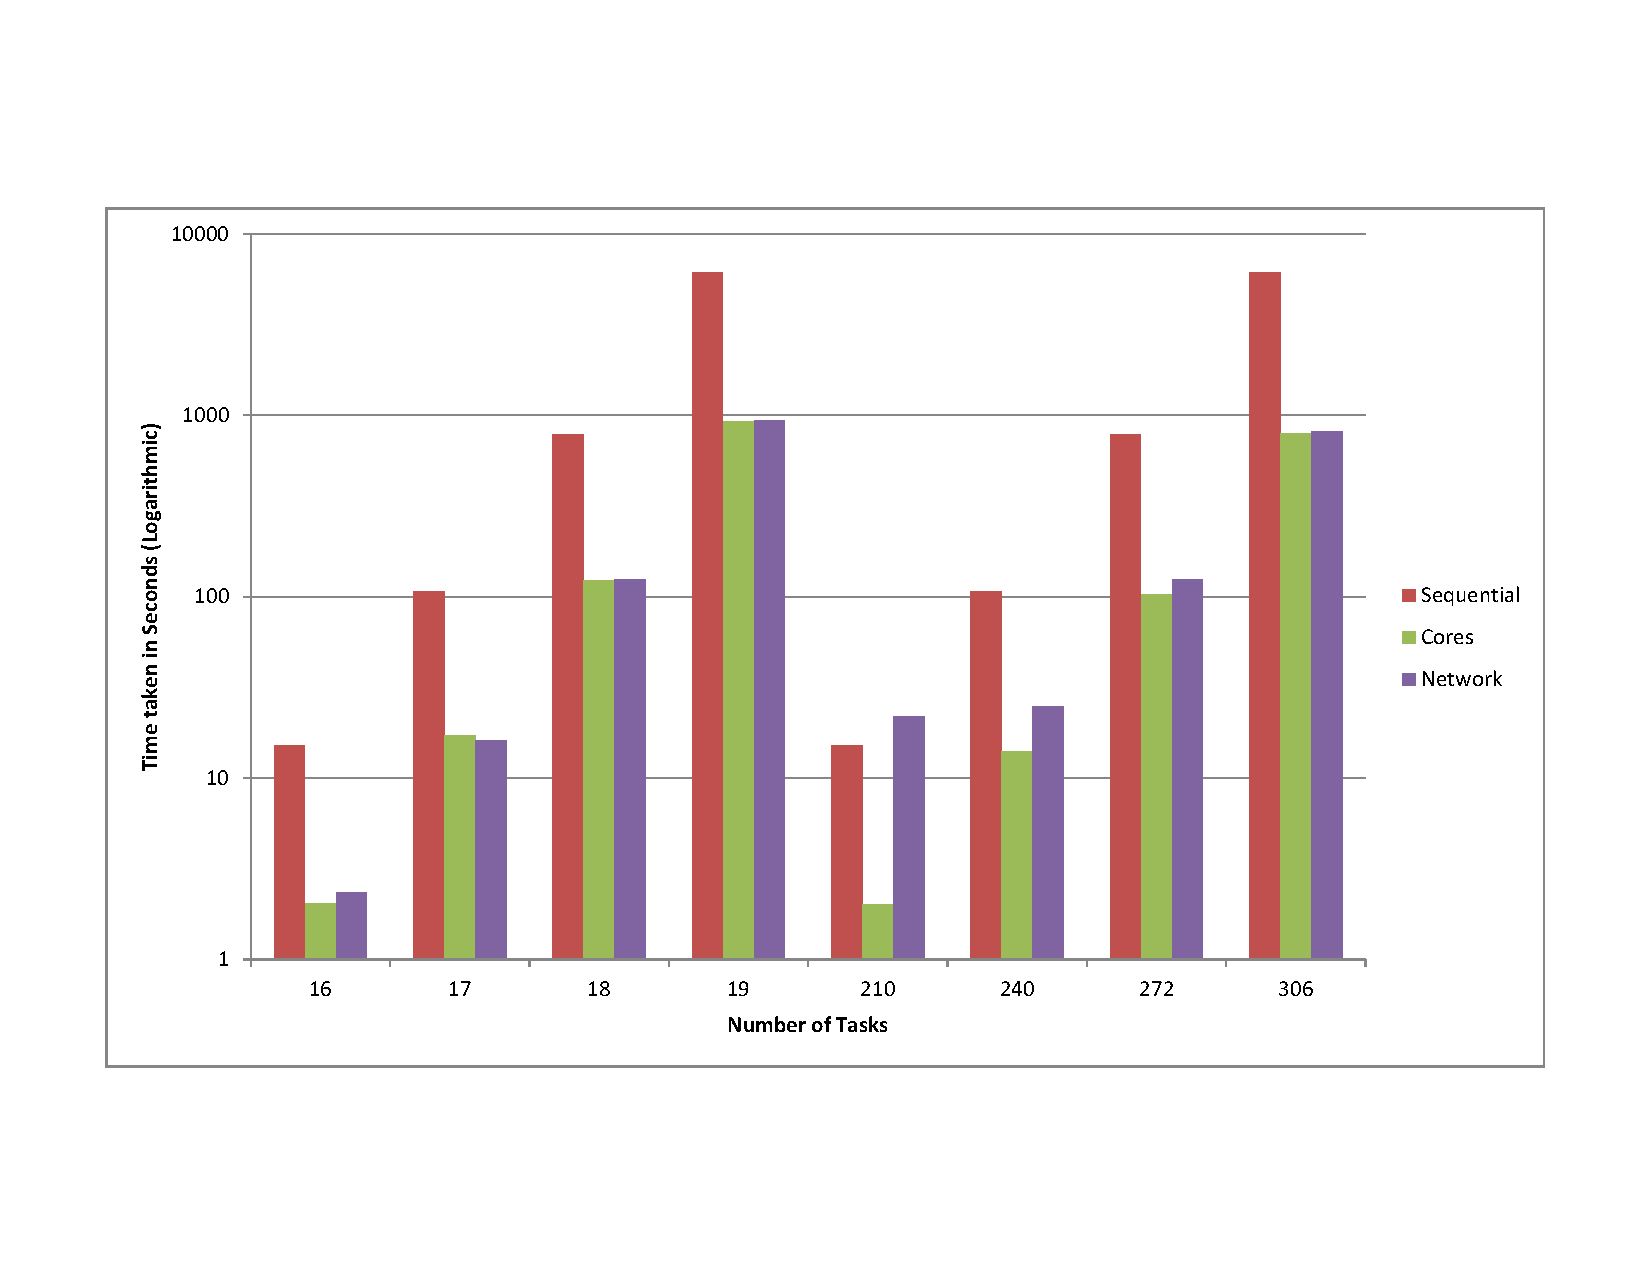
\includegraphics[width=\textwidth]{chart1.pdf}
  \end{center}
  \vspace*{-5em}
  \caption{Speedup ratios for the $N$-queens experiment.}
\label{fig:queens}
\end{figure}
From the table above and Fig.~\ref{fig:queens},
it is clear that the \of{Cores} and \of{Network}
implementations provide a significant speedup. As evident from the
last row, the speedup is almost 8, which is also the number of
cores we use.  It is also evident from the last column that the
\of{Network} implementation performs significantly better when the
computation time dominates in the total execution time.  The two extreme
cases correspond to the second and the last row: in the second row, the
communication time dominates and is in fact more than 91\%\ of the
total execution time; on the other hand, for the last row
communication time amounts to just 4.6\%\ of the total execution time.
As expected, the network implementation is only beneficial when the
computation time for each individual task is significant, which is the
case in realistic examples.

\subsection{Matrix Multiplication}\label{sec:matrix}

This benchmark was inspired by the PASCO'10 programming contest~\cite{PASCO}.
It consists of multiplication of
two square matrices of dimension 100 with integer coefficients.
Coefficients have several thousands of digits, hence we use
GMP~\cite{GMP} to handle operations over coefficients.

We compare the performances of two different implementations. In the
first one, called \of{mm1}, each task consists of the computation of a single
coefficient of the resultant matrix. 
In the second one, called \of{mm2}, each task consists of the
computation of a whole row of the resultant matrix.
As a consequence, the total number of tasks is
$10,000$ for \of{mm1} and only $100$ for \of{mm2}.
On the contrary, each task result for \of{mm1} is a single integer,
while for \of{mm2} it is a row of 100 integers.
%
The experimental results (in seconds) are tabulated below.
\begin{center}
  \begin{tabular}{|r|r|r|}
    \hline
    & \of{mm1}       & \of{mm2}  \\
    & (10,000 tasks) & (100 tasks) \\
    \hline\hline
\of{Sequential} & 20.3 &  20.2 \\
\hline
 \of{Cores} 
 (2 cores)     &   22.7 (0.89$\times$) &  11.3 (1.79$\times$) \\
 (4 cores)     &   12.3 (1.65$\times$) &   6.1 (3.31$\times$) \\
 (6 cores)     &    8.6 (2.36$\times$) &   4.3 (4.70$\times$) \\
 (8 cores)     &    8.0 (2.54$\times$) &   3.5 (\underline{5.77}$\times$) \\
 \hline
  \end{tabular}
\end{center}
The difference in the number of tasks explains the differences in the
speedup ratios above.
We do not include results for the network configuration, as they do
not achieve any benefit with respect to the sequential
implementation. The reason is that the communication cost dominates the
computation cost in such a way that the total execution time is
always greater than 30 seconds. Indeed, irrespective of the
implementation (\of{mm1} or \of{mm2}), the total size of the
transmitted data is $10^6$ integers, which in our case amounts to
billions of bytes.

A less naive implementation would have the worker read the input matrices
only once, \emph{e.g.} from a file, and then have the master send only
row and column indices. This would reduce the amount of transmitted data to
$10,000$ integers only.

%             mm1     mm2

% # tasks    10,000   100

% sequential  20.3   20.2

% cores 2     22.7   11.3
% cores 4     12.3    6.1
% cores 6      8.6    4.3
% cores 8      8.0    3.5

% network = workers on moloch + master on belzebuth

% cores 2     93     32.3
% cores 4     87     33.7
% cores 6     92     33.5
% cores 8     88     32.5

\begin{comment}
  As a first example, let us consider matrix multiplication.  We
  assume two matrices \of{a} and \of{b}, respectively of size
  $\of{n}\times\of{p}$ and $\of{p}\times\of{m}$, given as input, as
  well as a matrix \of{c} of size $\of{n}\times\of{m}$ to store the
  result.  Assuming \of{a} being a row-matrix and \of{b} a
  column-matrix, the standard matrix multiplication would be as
  follows:
  \begin{ocaml}
    for i = 0 to n-1 do for j = 0 to m-1 do for k = 0 to p-1 do
    c.(i).(j) <- c.(i).(j) + a.(i).(k) * b.(j).(k) done done done
  \end{ocaml}
  and runs in $O(\of{n}\times\of{p}\times\of{m})$, assuming addition
  and multiplication over coefficients to be denoted $+$ and $\times$
  respectively.  An easy way to distribute this computation is
  obviously to turn each computation of the inner loop over \of{k}
  into a task.  To do so, we first prepare the list of tasks:
  \begin{ocaml}
    let tasks = let l = ref [] in for i = 0 to n-1 do for j = 0 to m-1
    do tasks := ((a.(i), b.(j)), (i,j)) :: !tasks done done; !l
  \end{ocaml}
  Each task consists of row \of{a.(i)} and column \of{b.(j)} as first
  tuple, together with position \of{(i,j)} as a second tuple.  The
  worker is receiving the first tuple as argument and computes the dot
  product:
  \begin{ocaml}
    let worker (ai, bj) = let c = ref 0 in for k = 0 to p-1 do c := !c
    + ai.(k) * bj.(k) done; !c
  \end{ocaml}
  The master is a one line function which receives the result \of{r}
  from the worker and simply stores it into \of{c}, according to the
  position contained in the input task. It produces no new task.
  \begin{ocaml}
    let master (_, (i,j)) r = c.(i).(j) <- r; []
  \end{ocaml}
  Finally, the overall computation is started by invoking \of{compute}
  as follows:
  \begin{ocaml}
    let () = compute ~worker ~master !tasks
  \end{ocaml}
  The total number of tasks is $\of{n}\times\of{m}$.

  Using the sequential implementation provided by \of{Functory} is as
  simple as including the following line in the code:
  \begin{ocaml}
    open Sequential
  \end{ocaml}
  Then the computation is roughly similar to the standard
  multiplication described above.

  Now, let us assume we want to make use of a 4-core machine to
  perform the same computation.  This is achieved by just replacing
  the line above by
  \begin{ocaml}
    open Cores let () = set_number_of_cores 4
  \end{ocaml}
  while the rest of the code remains unchanged.

  Later, we may want to use a network of machines instead, for example
  two machines called \texttt{orcus} and \texttt{belzebuth} with 4 and
  8 cores respectively. Similar to the above, we turn the above lines
  into
  \begin{ocaml}
    open Network let () = declare_workers ~n:4 "orcus" let () =
    declare_workers ~n:8 "belzebuth" open Same
  \end{ocaml}
  Here, \of{Same} is a module which is to be used when master and
  worker are running the same executable. It provides a \of{compute}
  function which has the same signature as in modules \of{Sequential}
  and \of{Cores}, so that the rest of the code remains
  unchanged. Master and worker processes are distinguished at runtime
  using an environment variable \texttt{WORKER} which is set/unset.

  If we need to write two different programs for master and worker,
  for reason of binary incompatibility or any other reason, the
  library API is providing functions to do that. If master and worker
  are still compiled with the same version of \Ocaml, we use the
  \of{Poly} module which provides a polymorphic API. Let us start with
  the worker program.  It now looks like:
  \begin{ocaml}
    open Poly let worker (ai, bj) = ...  let () = Worker.compute
    worker ()
  \end{ocaml}
  The \of{Worker.compute} function enters a loop which waits for tasks
  sent by the master and returns results computed using \of{worker}.
  The master program is almost the same as before. First, we replace
  module \of{Same} with module \of{Poly}:
  \begin{ocaml}
    open Network let () = declare_workers ~n:4 "orcus" let () =
    declare_workers ~n:8 "belzebuth" open Poly
  \end{ocaml}
  Tasks and \of{master} function are unchanged:
  \begin{ocaml}
    let tasks = ...  let master (_, (i,j)) r = ...
  \end{ocaml}
  Finally, we start the computation with \of{Master.compute}, which
  does not have a \of{worker} parameter anymore:
  \begin{ocaml}
    let () = Master.compute ~master tasks
  \end{ocaml}

  When master and worker programs are compiled with different versions
  of the \Ocaml\ compiler, our library still provides a monomorphic
  API over strings. As a consequence, we need to convert tasks and
  results to and from strings in both master and worker.  The modified
  worker program then looks as follows:
  \begin{ocaml}
    open Mono let worker (ai, bj) = ...  let worker_string s =
    string_of_coeff (worker (task_of_string s)) let () =
    Worker.compute worker_string ()
  \end{ocaml}
  The master program is modified in a similar way.  We simply replace
  \of{Poly} with \of{Mono} and encode/decode coefficients as strings,
  as follows:
  \begin{ocaml}
    let tasks = ... string_of_task ...  let master (_, (i,j)) r =
    c.(i).(j) <- coeff_of_string r; []
  \end{ocaml}
  where \of{string_of_task} and \of{task_of_string} are user-defined
  functions to convert tasks to and from strings.
\end{comment}

\subsection{Mandelbrot Set}

Drawing the Mandelbrot set is another classical example that could be
distributed easily, since the color of each point can be computed
independently of the others. 
This benchmark consists in drawing the fragment of the Mandelbrot set
with lower left corner $(-1.1, 0.2)$ and upper right corner $(-0.8,
0.4)$, as a $9,000\times6,000$ image. 
%
If the total number of tasks $\of{t} \ge 1$ is given as a
parameter,  it is straight forward to split the image into \of{t} sub-images,
each of which is computed in parallel with and independently of the
others. In our case, the image is split into horizontal slices.
Each task is thus four floating-point numbers denoting the region
coordinates, together with two integers denoting the dimensions of the
sub-image to be drawn. The result of the task is a matrix of pixels,
of size $54,000,000 / \of{t}$. 
For instance, using $\of{t}=20$ tasks will
result in 20 sub-images of size $10.3$ Mb each,
assuming each pixel is encoded in four bytes.

The sequential computation of
this image consumes 29.4 seconds. For \of{Cores} and \of{Network}
implementations, the computation times in seconds are tabulated below.

% TODO compute ratios for Network
\begin{center}
  \begin{tabular}{|r|r|r|r|r|}
    \hline
    \#cores  &\#tasks & \of{Cores} & \of{Network} \\
    \hline\hline
    2       & 10 & 15.8       (1.86$\times$) &  20.3  (1.45$\times$)      \\
            & 30 & 15.7       (\underline{1.87}$\times$) &  18.7 (1.57$\times$)       \\
            & 100 & 16.1      (1.83$\times$) &  19.8   (1.48$\times$)    \\
            & 1000 & 19.6     (1.50$\times$) &  38.6    (0.76$\times$)  \\
    \hline
    4       & 10 & 9.50       (3.09$\times$)  &  14.4     (2.04$\times$)  \\
            & 30 & 8.26       (\underline{3.56}$\times$)  &  11.4  (2.58$\times$) \\
            & 100 & 8.37      (3.51$\times$)  &  11.4  (2.58$\times$) \\
            & 1000 & 10.6     (2.77$\times$)  &  20.5   (1.43$\times$) \\
    \hline
    8       & 10 & 9.40       (3.13$\times$)  &  12.6    (2.33$\times$)  \\
            & 30 & 4.24       (\underline{6.93}$\times$)  &   7.6  (3.87$\times$)    \\
            & 100 & 4.38      (6.71$\times$)  &   7.5    (3.92$\times$)  \\
            & 1000 & 6.86     (4.29$\times$)  &  11.3    (2.60$\times$)  \\
    \hline
  \end{tabular}
\end{center}
The best timings are achieved for the \of{Cores} configuration, where
communications happen within the same machine and are thus cheaper.
There are two significant differences with respect to the n-queens
benchmark.  On one hand, the number of tasks can be controlled more
easily than in the case of n-queens. We experimentally figured out the
optimal number of tasks to be 30. On the other hand, each computation
result is an image, rather than just an integer as in the case of
n-queens. Consequently, communication costs are much greater. 
In this particular experiment, the total size of the results
transmitted is more than 200 Mb.

\subsection{SMT Solvers}\label{sec:SMT}

Here we demonstrate the potential of our library for our application
needs as mentioned in the introduction. 
We consider 80 challenging verification conditions
(VC) obtained from the Why platform~\cite{filliatre07cav}.  Each
VC is stored in a file, which is accessible over
NFS. The purpose of the experiment is to check the validity of each VC
using several automated provers (namely Alt-Ergo, Simplify, Z3 and CVC3).

The master program proceeds by reading the file names, turning them
into tasks by multiplying them by the number of provers, resulting in
320 tasks in total.
Each worker in turn invokes the given prover on the given file, within
a timeout limit of 1 minute.
Each task completes with one of the four possible outcomes: \emph{valid},
\emph{unknown} (depending on
whether the VC is valid or undecided by the prover), 
\emph{timeout} and \emph{failure}.
The result of each computation is a pair denoting the status and the
time spent in the prover call. The master collects these results and
sums up the timings for each prover and each possible status.

Our computing
infrastructure for this experiment consists of 3 machines with 4, 8 and 8 cores
respectively, the master being run on a fourth machine. 
The figure below shows the total time in minutes spent by each prover
for each possible outcome.
\begin{center}
  \begin{tabular}{|r||r|r|r|r|}
    \hline
    prover   & valid & unknown & timeout & failure
    \\\hline\hline
    Alt-ergo & 406.0 & 3.0   &  11400.0 & 0.0       
    \\\hline
    Simplify &  0.5   & 0.4   &  1200.0 & 222.0   
    \\\hline
    Z3       & 80.7   & 0.0   &  1800.0 & 1695.0   
    \\\hline
    CVC3     & 303.0  & 82.7  &  4200.0 & 659.0   
    \\\hline
  \end{tabular}
\end{center}

These figures sum up to more than 6 hours if provers were executed
sequentially. However, using our library and our 3-machine
infrastructure, it completes in 22 minutes and 37 seconds, giving us a
speedup of more than 16$\times$. We are still far away from the ideal
ratio of 20$\times$ (we are using 20 cores), since some provers are
allocating a lot of memory and time spent in system calls is not
accounted for in the total observed time. However, a ratio of
16$\times$ is already a significant improvement for our day-to-day
experiments. Further a large parallelizable computation could be
distributed by just adding 3-4 lines of code (to just specify the
module to be used and the tasks) which is an important user-friendly
feature of the library. Further we assume files available over
NFS. Intelligent distribution of data over a network is in itself an
area of research which is beyond the scope of our work.

\section{Conclusions and Future Work}\label{sec:future}

In this paper, we presented a distributed programming library for
\Ocaml. The main features are the
genericity of the interface, which makes use of polymorphic
higher-order functions, and the ability to easily switch between
sequential, multi-core, and network implementations. In particular,
\functory\ allows to use the same executable for master and workers,
which makes the deployment of small programs immediate --- master and
workers being only distinguished by an environment
variable. \functory\ also allows master and workers to be completely
different programs, which is ideal for large scale deployment.
Another distinguishing feature of our library is a robust
fault-tolerance mechanism which relieves the user of cumbersome
implementation details.  Yet another interesting feature of the
library is the ability to add workers dynamically. \functory\
also allows to cascade several distributed computations inside the
same program.  Finally, the low-level API of \functory\ 
can be used to write interactive programs where one can adjust certain
parameters in a GUI, like increasing or decreasing the number of
workers, to observe the progress in computation, resource consumption, etc.

\paragraph{Future Work.}
There are still some interesting features that could be added to our
library. 
\begin{itemize}
\item 
  One is the ability to efficiently assign tasks to workers depending
  on resource parameters, such as data locality, CPU power, memory,
  etc. This could be achieved by providing the user with the means to control
  task scheduling.  This would enable \functory\ to scale up to
  MapReduce-like applications.

  Currently, without any information about the tasks, the scheduling
  is completely arbitrary. In both \of{Cores} and \of{Network}
  modules, we use traditional queues for the pending tasks; in
  particular, new tasks produced by the master are appended to the end
  of the queue.

% \item 
%   Another interesting feature could be the ability
%   to add or remove machines dynamically. Currently, our library assumes
%   that the list of machines to be used is given \emph{a priori}, as
%   part of the code. An alternative would be to read machine names from
%   a file, watched periodically by the master.
\item
  Our library provides limited support for retrieving real-time
  information about computations and communications. Processing and storing
  information about workers and tasks locally in the master is
  straightforward.
 
\item 
  One very nice feature of Google's MapReduce is the possibility to
  use redundantly several idle workers on the same tasks
  for speedup when reaching the end of computation.
  Since we already have the fault-tolerance implemented, this
  optimization should be straightforward to add to our library.
\end{itemize}
We intend to enrich our library with all above features.

%\appendix

\paragraph{Acknowledgments.}
We are grateful to the ProVal team for support and comments
on early versions of the library and of this paper.
We thank the anonymous reviewers for their helpful comments and
suggestions.

%\vfill\pagebreak
%\bibliographystyle{plain}
%\bibliography{./biblio}
\begin{thebibliography}{10}

\bibitem{camlP3l}
{CamlP3l}.
\newblock \url{http://camlp3l.inria.fr/}.

\bibitem{plasma}
{Plasma}.
\newblock \url{http://plasma.camlcity.org/plasma}.

\bibitem{erlang}
{The Erlang Programming Language}.
\newblock \url{http://www.erlang.org/}.

\bibitem{GMP}
{The GNU Multiple Precision Arithmetic Library}.
\newblock \url{http://gmplib.org/}.

\bibitem{PASCO}
{Parallel Symbolic Computation 2010 (PASCO)}, 2010.
\newblock \url{http://pasco2010.imag.fr/}.

\bibitem{mapreduce}
Jeffrey Dean and Sanjay Ghemawat.
\newblock {MapReduce: Simplified Data Processing on Large Clusters}.
\newblock In {\em OSDI}, pages 137--150, 2004.

\bibitem{filliatre07cav}
Jean-Christophe Filli\^atre and Claude March\'e.
\newblock {The {Why/Krakatoa/Caduceus} Platform for Deductive Program
  Verification}.
\newblock In Werner Damm and Holger Hermanns, editors, {\em 19th International
  Conference on Computer Aided Verification}, volume 4590 of {\em Lecture Notes
  in Computer Science}, pages 173--177, Berlin, Germany, July 2007. Springer.

\bibitem{iTask}
Jan~Martin Jansen, Rinus Plasmeijer, Pieter Koopman, and Peter Achten.
\newblock {Embedding a Web-based Workflow Management System in a Functional
  Language}.
\newblock In {\em Proceedings of the Tenth Workshop on Language Descriptions,
  Tools and Applications}, LDTA '10, pages 7:1--7:8, New York, NY, USA, 2010.
  ACM.

\bibitem{ocamlMPI}
Xavier Leroy.
\newblock {OCamlMPI: Interface with the MPI Message-passing Interface}.
\newblock \url{http://pauillac.inria.fr/~xleroy/software.html}.

\bibitem{mandel2008}
Louis Mandel and Luc Maranget.
\newblock Programming in {JoCaml} (tool demonstration).
\newblock In {\em 17th European Symposium on Programming ({ESOP 2008})}, pages
  108--111, Budapest, Hungary, April 2008.

\bibitem{ML5}
Tom Murphy, VII., Karl Crary, and Robert Harper.
\newblock {Type-safe Distributed Programming with ML5}.
\newblock In {\em Proceedings of the 3rd conference on Trustworthy global
  computing}, TGC'07, pages 108--123, Berlin, Heidelberg, 2008.
  Springer-Verlag.

\bibitem{poor-man-mapreduce}
Yoann Padioleau.
\newblock {A Poor Man's MapReduce for OCaml}, 2009.
\newblock \url{http://www.padator.org/ocaml/mapreduce.pdf}.

\bibitem{GdH}
Robert~F. Pointon, Philip~W. Trinder, and Hans-Wolfgang Loidl.
\newblock {The Design and Implementation of Glasgow Distributed Haskell}.
\newblock In {\em Selected Papers from the 12th International Workshop on
  Implementation of Functional Languages}, IFL '00, pages 53--70, London, UK,
  2001.

\end{thebibliography}

\end{document}

% LocalWords:  parallelize functor parameterized indices endianness monomorphic
% LocalWords:  genericity executables OCamlMPI MapReduce marshaling functors
% LocalWords:  workflow combinators granularities
